\chapter{Casos de estudio}
\label{ch7:examples}

A continuaci\'on, se aplican los resultados de los cap\'itulos anteriores a dos casos particulares.
El primer caso fue tomado del art\'iculo de \citet{mendoza-torres_bernstein_2017}. 
En \'el se muestra la aplicaci\'on a una red de fracturas considerando solamente la dependencia entre la orientaci\'on y la longitud.
La aplicaci\'on trivariada (orientaci\'on-longitud-apertura) se muestra en el segundo caso.

\section{Caso bivariado orientaci\'on-longitud}

\subsection{Descripci\'on de los datos}
\label{ss:synthData}

Aunque la metodolog\'ia es v\'alida para cualquier sistema de fracturas, en esta secci\'on se presenta una red de fracturas cuyo comportamiento es frecuentemente encontrado dentro de la corteza terrestre. Debido a la falta de datos reales, se gener\'o un conjunto de datos tratando de reproducir cierto conocimiento geol\'ogico:

% Extension fracture
\setlength{\epigraphwidth}{0.9\textwidth}
\epigraph{\textit{Fracura de extensi\'on}: Fractura formada por la extensi\'on perpendicular a las paredes de la fractura. La magnitud de la extensi\'on puede ser min\'uscula como en el caso de 
\textit{juntas}, o puede ser tan grande como las \textit{venas}}{\citet[p. 434]{fossen_structural_2010}}

\setlength{\epigraphwidth}{0.9\textwidth}
\epigraph{las juntas de cizalla comunmente ocurren en \textit{conjuntos conjugados}\ldots las juntas de cizalla ocurren en conjuntos conjugados oblicuos en donde las juntas de extensi\'on aparecen como juntas longitudinales y transversas que un par ortogonal}{\citet[p. 17]{singhal_applied_2010}}
%singhal_applied_2010 "Shear joints ... forming an orthogonal pair (Fig. 2.7)."

A\'un m\'as, algunos sistemas de fracturas tienen relaciones espec\'ificas de orientaci\'on y longitud:

\setlength{\epigraphwidth}{0.9\textwidth}
\epigraph{Los mineros se refieren a estas fracturas en direcciones caracter\'isticas como \textit{cruceros de carb\'on}: un crucero constituido por por face cleats, largas fracturas dominantes (juntas sistem\'aticas) que pueden extenderse por varios metros de manera horizontal; y por, butt cleats, otro conjunto de fracturas m\'as cortas escasamente desarrolladas que terminan en las face cleats en \'angulos rectos (juntas transversales).}{\citet{davis_structural_2011}}
%2012-Structural geology of rocks and regions (Davis, Raynolds and Kluth), page 241: "Miners refer to these two distinctive fracture directions as coal cleats: a face cleat composed of long continuous dominant fractures (systematic joints) that extend for many meters horizontally; and a butt cleat composed of shorter, somewhat more poorly developed fractures that terminate at right angles against the face cleat (cross joints)... “Scatter” in the orientations of the face cleats is related primarily to the influence of local stresses, which can cause shifts of joint trends from the direction(s) predicted by the regional orientation of far-field stresses, and which at a much finer scale can cause shifts in orientations of parts of individual joint surfaces." "Jointing Associated with Large Individual Folds" "It is not uncommon for faults to occur in conjugate sets (Figure 6.66A) that intersect in an acute angle, commonly 60"
%1998 Laubach, Marrett, Olson, Scott Characteristics and origins of coal cleat. "cleat lengths and heights are reported to range from microns to meters. Tremain et al., 1991.Yet these cleats are arranged in a hierarchy of sizes that includes fractures of decimeter size 'master cleats', Fig. 1."

% Rose diagrams of coal cleats:
%2004_Gillam, Flottmann and Hillis_Natural fracture characterisation in a coal measure succession. an analogue for coal seam methane and tight gas reservoirs
%2006 the nature of naturally fractured reservoir schlumberger
%2008_ Pashin, Jin, Zheng_2Discrete Fracture Network Models for Risk Assessment of Carbon Sequestration in Coal

%Usually, fractures form as conjugate sets \cite{}[section 2.2.3.5, and fig. 2.9] 2010-Applied Hydrogeology of Fractured Rocks (Singhal and Gupta)."the observed length of fracture trace depends on the relative orientation between the fracture plane and the exposure face"

Para mayor detalle y datos en los que se basa esta afirmaci\'on sobre los cruceros de carb\'on cons\'ultese los art\'iculos de \citet{rodrigues_coal_2014}; \citet{laubach_characteristics_1998}; y \citet{datta_coal_2016}. 

A partir de este conocimiento de la geolog\'ia estructural, el conjunto de datos de orientaci\'on y longitud a estudiar debe satisfacer:

\begin{itemize}
	\item Tener dos familias $f90$ y $f0$, siendo esta \'ultima la familia dominante, es decir, con fracturas m\'as largas.
	%	see FIGURE 5 of http://www.cdc.gov/niosh/mining/userfiles/works/pdfs/ri7910.pdf
	\item las longitudes de la familia $f90$ son menores que la familia conjugada.
	\item La familia en la direcci\'on Este ($f90$), con fracturas m\'as peque\~nas, debe tener m\'as fracturas que la familia dominante.
	%	\item length distribution is bimodal? No always, look for references.
	%"Renshaw, 1999, Conectivity..."
	%1997 Clemo, Smith _ A hierarchical model for solute transport in fractured media
	%	\item f0 is more disperse than f90? look for references
\end{itemize}

Nos referiremos al conjunto de datos a estudiar como \textit{los datos}, o los \textit{datos sint\'eticos}, y ser\'an considerados como si fueran reales. Estos 400 datos se componen de las coordinadas cartesianas de los centros de fracturas $\vec{x} = (x,y) \in [0,400] \times [0,400]$.
Debido a razones de visualizaci\'on y comparaci\'on, estos centros de fracturas se obtuvieron con un proceso homog\'eneo de Poisson con intensidad $\theta = 1$.
Las direcciones de rumbo de las fracturas fueron muestreadas de una combinaci\'on de dos distribuciones de von Mises con par\'ametros mostrados en la \autoref{t:movMpar}.
Estos \'angulos se encuentran en el rango $[0, 180)$ en un sistema de coordenadas geogr\'afico (Norte = 0$^{\circ}$, Este = 90$^{\circ}$).
Las longitudes fueron muestreadas mediante una distribuci\'on lognormal.
Aunque generalmente las fracturas muestran un comportamiento auto-af\'in por lo que se observan de manera similar a varias escalas; atendiendo a las citas geol\'ogica de \citet{davis_structural_2011} en este trabajo, utilizaremos cm para las longitudes de fracturas.

Con respecto a la estructura de dependencia, los datos anteriores se muestrearon pegando dos c\'opulas (gluing copulas) de Placket (\verb|copBasic::PLACKETTcop|). Para pseudo-observaciones en el intervalo $u_{\theta} = [0, 0,5)$, se utiliz\'o una dependencia aproximadamente lineal y directa (par\'ametro de placket = $0.06$); para las pseudo-observaciones en el intervalo $u_{\theta} = [0.5, 1]$ se utiliz\'o una dependencia aproximadamente lineal e inversa (par\'ametro de placket = $20$). Esta estructura de dependencia se puede observar en la \autoref{f:scatterplot}.

Como resultado, la red de fracturas discretas en ser analizadas y modelada con la metodolog\'ia est\'andar y conjunta se muestra en la \autoref{f:dfn}. En esta figura, para analizar la relaci\'on de dependencia entre direcci\'on y longitud, se colorearon en negro las fracturas con longitudes mayores a 51 cm mientras que las fracturas menores en azul claro. Este corte se bas\'o en el 90$^\circ$ percentil del modelo de longitudes. Es decir, aproximadamente el 10\% del total de fracturas son negras.

\begin{figure} % Parameters meaning: https://www.sharelatex.com/learn/Positioning_images_and_tables#Positioning_tables
	\centering
	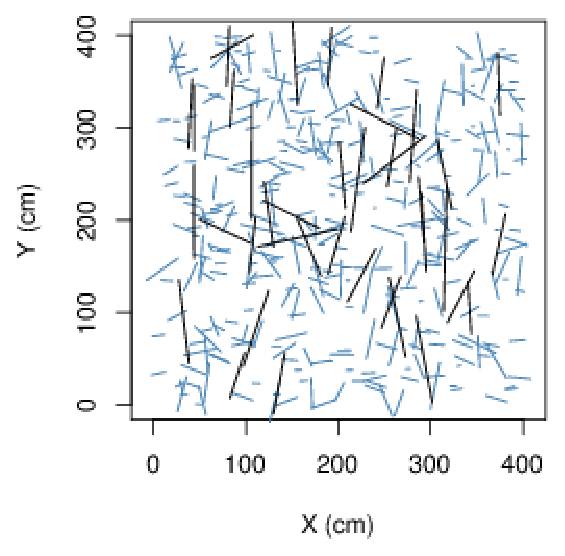
\includegraphics{fig2}
	\caption{Representaci\'on gr\'afica de la red de fracturas de los datos sint\'eticos. Aproximadamente el 10\% de las fracturas son de color negro.}
	\label{f:dfn}
\end{figure}

Las orientaciones fueron generadas usando la funci\'on \verb|rmixedvonmises| del paquete \verb|circular| \citep{agostinelli_r_2013} con los par\'ametros de la \autoref{t:movMpar}. En la \autoref{t:circStats} se muestran algunos de sus estad\'igrafos, calculados con el mismo paquete.
La media circular (89.7$^{\circ}$) es muy similar a la mediana
(88.5$^{\circ}$). Ambos estad\'igrafos muy parecidos a la familia f90. El valor muy peque\~no de asimetr\'ia es un indicador de que la distribuci\'on es altamente sim\'etrica. Estos resultados tambi\'en se pueden visualizar en la \autoref{f:rose}, la cual muestra que la familia f90 tiene una poblaci\'on mayor que la familia en la direcci\'on N-S. \'Esta \'ultima observaci\'on en total acuerdo con los requerimientos del modelo.

\begin{table}[H]
	\centering
	\begin{tabular}{ |c|c|c|c|}
		\hline
		familia & proporci\'on & $\mu (^{\circ}$) & $\kappa$ \\ \hline
		f0     &    0.3     &   0   & 10       \\ \hline
		f90    &    0.7     &  90   & 10       \\ \hline
	\end{tabular}
	\caption{Par\'ametros de la combinaci\'on de dos distribuciones de von Mises de donde fueron muestreadas las 400 direcciones de la red de fractura a modelar.}
	\label{t:movMpar} % stands for "Table" of 'm'ixture 'o'f two 'v'on 'M'ises distributiions 'par'ameters
\end{table}


\begin{figure}[H]
	\centering
	\includegraphics{fig3}
	\caption{Roseta de los datos a analizar. f0 est\'a en la direcci\'on N-S, f90 en la direcci\'on perpendicular (E-O).}
	\label{f:rose}
\end{figure}

\begin{table}[H]
	\centering
	\begin{tabular}{ |c|c|}
		\hline
		Estad\'igrafo         &  valor   \\ \hline\hline
		Mediana             & 88.458$^{\circ}$ \\ \hline
		$\mu$              & 89.728$^{\circ}$ \\ \hline
%		Longitud resultante   &  0.306   \\ \hline
		Desviaci\'on est\'andar &  44.063  \\ \hline
		Asimetr\'ia           &  0.045   \\ \hline
	\end{tabular}
	\caption{Estad\'istica circular de las direcciones de los datos sint\'eticos.}
	\label{t:circStats}
\end{table}



Las longitudes fueron generadas utilizando lo funci\'on \verb|rlnorm| del paquete \verb|stats|. Los par\'ametros de la distribuci\'on lognormal en dicha funci\'on son $meanlog = 3$, $sdlog= 0.73$, la media y la desviaci\'on est\'andar en la escala logar\'itmica. Los estad\'igrafos en la \autoref{t:lengthStats} muestran la diferencia entre los valores de la media y la mediana. Esto es una muestra de alta asimetr\'ia tambi\'en en la misma tabla. El histograma adem\'as muestra una peque\~na moda alrededor de los 70 cm.

\begin{figure}
	\centering
	\includegraphics[width=0.8\textwidth]{fig4}
	\caption{Histograma de las longitudes de fractura. La longitud se distribuye lognorm(meanlog = 3.00, sdlog = 0.73)}
	\label{f:hist}
\end{figure}

\begin{table}[H]
	\centering
	\begin{tabular}{ |c|c|}
		\hline
		Estad\'igrafo         & valor  \\ \hline\hline
		Mediana             & 20.389 cm \\ \hline
		Media               & 26.186 cm \\ \hline
		Desviaci\'on est\'andar & 20.894 cm \\ \hline
		Asimetr\'ia           & 1.914  \\ \hline
	\end{tabular}
	\caption{Estad\'igrafos de las longitudes de los datos sint\'eticos.}
	\label{t:lengthStats}
\end{table}



La \autoref{f:cdfDL} muestra las funciones de distribuci\'on acumulativa de la direcci\'on y de la longitud. Aunque estos datos tienen un comportamiento marcadamente diferente, la funci\'on cuantil de Bernstein-Kantorovich muestra representar bastante bien ambos comportamientos. Para los datos orientados, en este trabajo se prefiere la flexibilidad de dicha funci\'on cuantil en vez de 'ajustar artificialmente una funci\'on como la von Mises.

\begin{figure}
	\centering
	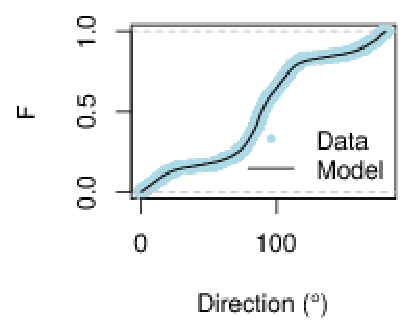
\includegraphics{fig5left}
	\qquad
	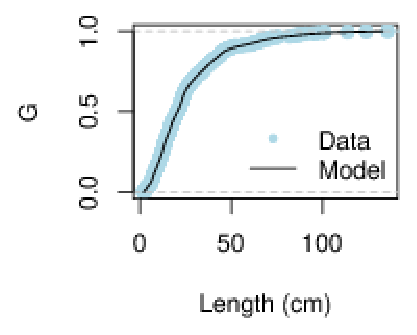
\includegraphics{fig5right}
	\caption{Funci\'on de distribuci\'on acumulativa y su respectivo modelo ajustado mediante la funci\'on cuantil de Bernstein-Kantorovich. Izquierda: direcci\'on; Derecha: longitud.}
	\label{f:cdfDL}
\end{figure}

El diagrama de dispersi\'on (\autoref{f:scatterplot}) direcci\'on-longitud y su correspondiente gr\'afico de pseudo-observaciones $uv$ se muestran para entender el comportamiento bivariado, es decir, para entender la estructura de dependencia subyacente. La diferencia entre ambos gr\'aficos reside en que el diagrama de dispersi\'on de los datos vive en el producto cartesiano de los rangos de las dos variables aleatorias mientras que el gr\'afico de pseudo-observaciones vive en el cuadrado unitario ($[0, 1] \times [0, 1]$).

Dado que el an\'alisis de dependencia utilizando la teor\'ia de c\'opula no es est\'andar fuera del \'ambito estad\'istico, expliquemos brevemente c\'omo se efect\'ua. Los valores en los ejes del gr\'afico de pseudo-observaciones \autoref{f:scatterplot} corresponden a las probabilidades (acumulativas) de los cuantiles (ejes en el diagrama de dispersi\'on). Por ejemplo, en el eje horizontal del diagrama de dispersi\'on (izquierda de \autoref{f:scatterplot}), el \'angulo 90$^\circ$ (la media) corresponde a $u = 0.5$ en el gr\'afico de pseudo-observaciones; mientras que el tercer cuantil en el diagrama de dispersi\'on corresponde a $u = 0.75$. El \'angulo 0$^\circ$ corresponde a $u=0$. De manera similar para el eje vertical.

El gr\'afico de pseudo-observaciones permite entender de manera visual la estructura de dependencia. De esta manera se puede estudiar el efecto que tiene la estructura de dependencia sobre el diagrama de dispersi\'on.

El coeficiente de correlaci\'on de rango para estos datos ($\rho_M = 0.635$) es un indicador de que la orientaci\'on no es independiente de la longitud. Este n\'umero fue calculado con los c\'odigos que se pueden encontrar en el trabajo de \citet{tu_study_2015}.

Un indicador m\'as confiable para determinar independencia se debe basar en la teor\'ia de c\'opulas. La funci\'on \verb|indepTest|  del paquete \verb|copula| permite hacer una prueba de independencia basada en c\'opulas. Para los datos en uso se obtuvo un estad\'istico de la prueba con valor 0.408 y un p-valor de 5\e{-4}, lo que indica que la independencia es rechazada. Por lo tanto, s\'i es \'util continuar con el modelado de la estructura de dependencia.

%The correlation coefficient were computed with the \verb|hoefCOP| function from the \verb|copBasic| package \citep{Asquith2015} and the codes provided in \citet{tu_study_2015}.

\begin{figure}[H]
	\centering
	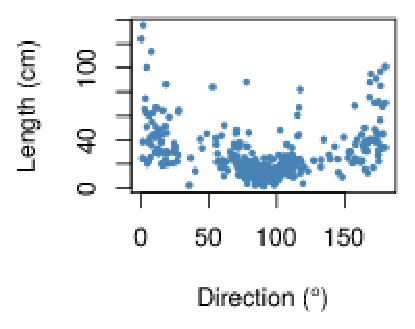
\includegraphics{fig6left}
	\qquad
	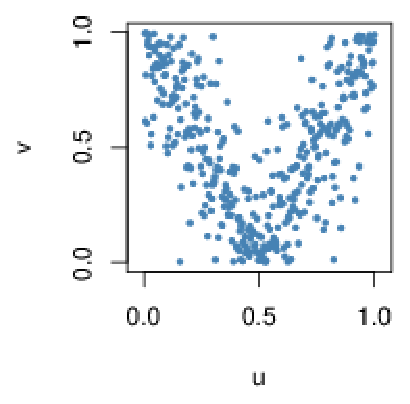
\includegraphics{fig6right}
	\caption{Diagrama de dispersi\'on de la longitud vs direcci\'on (izquierda), y su correspondiente gr\'afico de pseudo-observaciones (derecha).}
	\label{f:scatterplot}
\end{figure}

En el diagrama de dispersi\'on claramente se muestra una moda en la direcci\'on N-S pero la otra familia es casi indistinguible. Es decir, la familia f0 resalta m\'as que la familia f90. En contraste, en la roseta de direcciones sucede lo casi contrario. Ah\'i s\'i se pueden visualizar claramente ambas modas, pero la que m\'as resalta es la de la familia en la direcci\'on E-O. En el diagrama de dispersi\'on se puede observar que la probabilidad de obtener fracturas con longitudes menores a, digamos, 18cm, dentro de la familia N-S es casi cero. Un fen\'omeno inverso se puede observar en la familia E-O: muchas fracturas peque\~nas y casi ninguna grande.

\'Este fen\'omeno se debe a la estructura de dependencia mostrada en el gr\'afico de pseudo-observaciones. N\'otese tambi\'en que hay muchas m\'as fracturas peque\~nas (menores a 51 cm, por ejemplo) que fracturas largas a lo largo del rango de direcciones, $[0, 180^\circ$).

\subsection{La metodolog\'ia est\'andar}

Para el siguiente an\'alisis es conveniente distinguir entre las palabras 'sint\'etico' y simulado. Cuando usemos el primero ser\'a para referirnos al conjunto de datos de la secci\'on pasada. N\'otese pue para un conjunto de datos pueden existir m\'ultiples simulaciones.

En esta secci\'on se muestran resultados utilizando una metodolog\'ia cuasi-est\'andar. El t\'ermino \textit{cuasi} se debe a que no se hace clasificaci\'on de fracturas alguna ya que con la funci\'on cuantil de Bernstein-Kantorovich se puede modelar directamente datos multimodales. De esta manera, las funciones marginales univariadas son modelas de manera id\'entica que en la secci\'on siguiente. Esto nos permite ser m\'as objetivos en la comparaci\'on del an\'alisis bivariado, que en la metodolog\'ia est\'andar se hace simulando cada variable de manera independiente.

Los modelos marginales univariados utilizados ser\'an los mismos que en la \autoref{f:cdfDL}. Para facilitar la comparaci\'on, los anchos de clase son los mismos tanto en la roseta de direcciones de los datos sint\'eticos (\autoref{f:rose}) como en la delos datos simulados (\autoref{f:roseSim}. De manera similar para los histogramas de los datos sint\'etico y los simulados. De manera bivariada, los rangos tanto en el eje vertical como en el horizontal fueron fijados. Tambi\'en en la parte espacial, los centros de las fracturas son exactamente los mismos.

La roseta de las simulaciones independientes (\autoref{f:roseSim}) parece m\'as suavizada, es decir, comparando con la roseta de los datos (\autoref{f:rose}), hay menos contraste entre las modas y los valles. A diferencia de este comentario, las ubicaciones de dichas modas y valles son satisfactoriamente reproducidas. Incluso, una ligera asimetr\'ia alrededor de 90$^\circ$ es reproducida. De manera cuantitativa, los estad\'igrafos circulares (\autoref{t:circStatsSim}) tambi\'en muestra lo bueno que es el ajuste. Sin embargo, el aumento de desviaci\'on est\'andar remarca la sospecha del efecto de suavizado.

%For a comparison to the methodology of this work, \autoref{f:uvSimInd} shows the pseudo-observations of a simulation made with the standard methodology in which no dependendence is modeled. This figure corresponds to exactly the same marginal dataset $\{\theta_i, l_i\}$ as the simulation with dependence in \autoref{f:uvSim}, i. e, the mean, variance and other statistics are identical to those in \autoref{t:circStatsSim} and \autoref{t:lengthStatsSim} but the difference is the underlying copula.

%In \autoref{f:alSimInd} is shown the consequences in the scatterplot and the DFN of having the dependence structure of \autoref{f:uvSimInd}. Again, the 90th percentile (51cm) has been used as a cutoff to highlight the 10\% of the larger fractures. Notice the direction of these in the scatterplot and the DFN are more disperse (no preferred direction) than in the simulation taken into account the dependence structure (\autoref{f:dfnSim}).

\begin{figure}
	\centering
	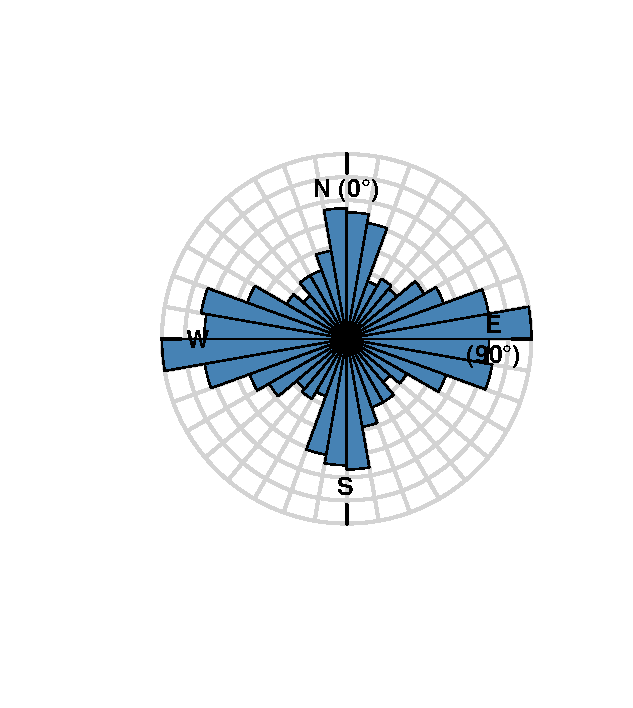
\includegraphics{fig7}
	\caption{Roseta de orientaciones de una simulaci\'on. Comp\'arese con \autoref{f:rose}}.
	\label{f:roseSim}
\end{figure}

\begin{table}[H]
	\centering
	\begin{tabular}{ |c|c|}
		\hline
		Estad\'igrafo         & valor  \\ \hline\hline
		Mediana             & 83.930$^{\circ}$  \\ \hline
		$\mu$              & 85.431$^{\circ}$ \\ \hline
%		Longitud resultante   & 0.233  \\ \hline
		Desviaci\'on est\'andar & 48.920 \\ \hline
		Asimetr\i'a           & 0.166 \\ \hline
	\end{tabular}
	\caption{Estad\'igrafos circulares de las direcciones de una simulaci\'on de los datos. Comp\'arese con \autoref{t:circStats}.}
	\label{t:circStatsSim}
\end{table}



Las longitudes, simuladas independientemente de las orientaciones, tambi\'en fueron reproducidos. N\'otese por ejemplo que el valle observado a aproximadamente 55cm se reproduce en es histograma (\autoref{f:histSim}). La moda sutil alrededor de los 70 cm tambi\'en aparece en esta simulaci\'on. Por el lado cuantitativo, la media y la mediana son distintos entre s\'i pero muy parecidos sus correspondientes en los datos sint\'eticos. Aqu\'i tambi\'en se muestra un aumento en la desviaci\'on est\'andar.

\begin{figure}
	\centering
	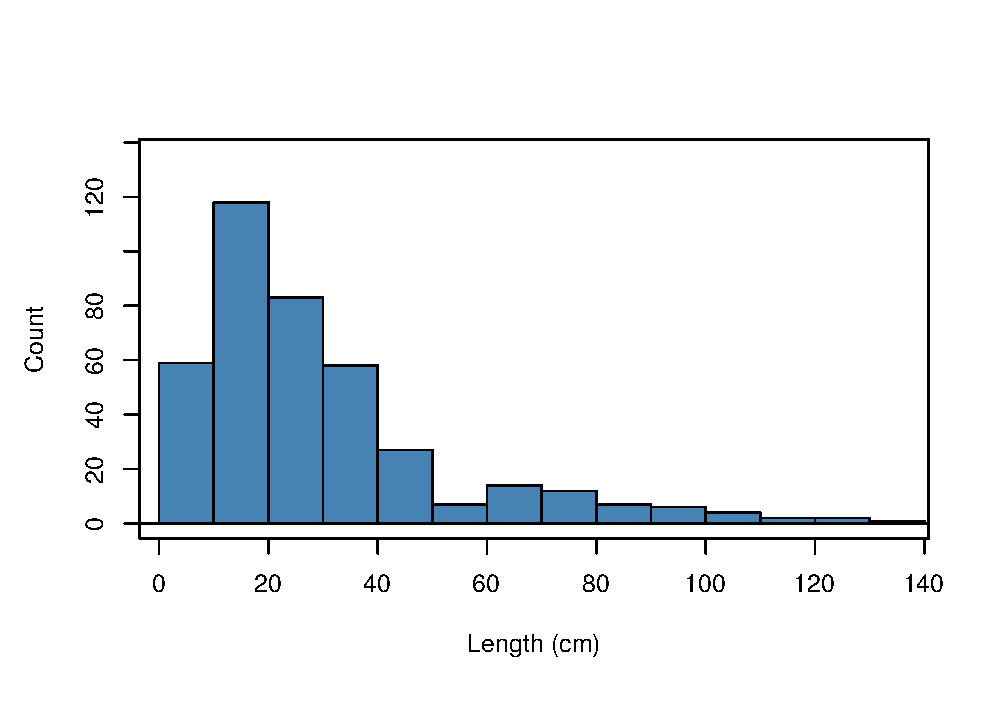
\includegraphics[width=0.8\textwidth]{fig8}
	\caption{Histograma de longitudes de una simulaci\'on. Comp\'arese con la \autoref{f:hist}.}
	\label{f:histSim}
\end{figure}

\begin{table}[H]
	\centering
	\begin{tabular}{ |c|c|}
		\hline
		Estad\'igrafo         & valor  \\ \hline\hline
		Mediana             & 22.877 cm \\ \hline
		Media               & 29.400 cm \\ \hline
		Desviaci\'on est\'andar & 23.930 cm \\ \hline
		Asimetr\i'a           & 1.752  \\ \hline
	\end{tabular}
	\caption{Estad\'igrafos de las longitudes de una simulaci\'on de los datos. Comp\'arese con la \autoref{t:lengthStats}.}
	\label{t:lengthStatsSim}
\end{table}



Esta coherencia entre la simulaci\'on y los datos tambi\'en se observa en la cercan\'ia de la funci\'on de distribuci\'on acumulativa emp\'irica con la de los modelos (\autoref{f:cdfLs}). \'Este es el resultado de la cualidad no-param\'etrica de la funci\'on cuantil de Bernstein-Kantorovich.

\begin{figure}[H]
	\centering
	\includegraphics{fig9left}
	\qquad
	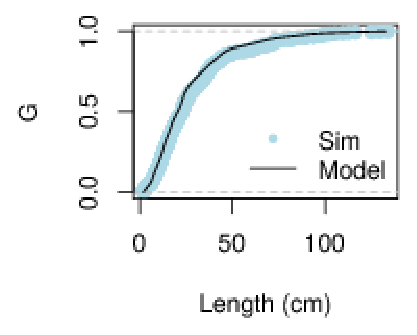
\includegraphics{fig9right}
	\caption{Funciones de distribuci\'on acumulativa emp\'irica de los datos y sus respectivos modelos. Izquierda: Direcciones; Derecha: longitudes.}
	\label{f:cdfLs}
\end{figure}

N\'otese sin embargo que en el caso bivariado (\autoref{f:alSimInd}) el modelado no es tan satisfactorio como en el caso univariado.
Tanto en el diagrama de dispersi\'on como en el gr\'afico de pseudo-observaciones los puntos est\'an m\'as dispersos, sin forma preferencial alguna.
Cuantitativamente, el coeficiente de correlaci\'on es claramente diferente ($\rho_M = 0.016$).
Ni el diagrama de dispersi\'on ni el gr\'afico de pseudo-observaciones muestra la estructura de los datos que se quiso modelar. La raz\'on: la simulaci\'on no tom\'o en cuenta ning\'un dato bivariado. La metodolog\'ia est\'andar siempre produce resultados como \'este gr\'afico de pseudo-observaciones: puntos distribuidos independientemente (\autoref{f:alSimInd}).

\begin{figure}[H]
	\centering
	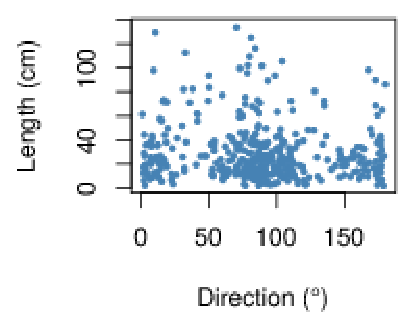
\includegraphics{fig10left}
	\qquad
	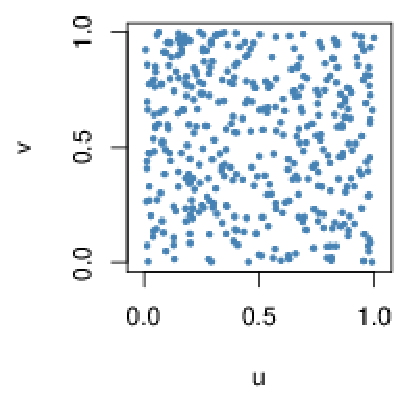
\includegraphics{fig10right}
	\caption{Diagramas de dispersi\'on de la simulaci\'on. Izquierda: los datos; derecha: las pseudo-observaciones.}
	\label{f:alSimInd}
\end{figure}

La DFN resultante paga el precio al mostrar, por ejemplo, que el 10\% de las fracturas m\'as largas no est\'an preferencialmente en la direcci\'on N-S como los datos originales. Al contrario, ahora las fracturas m\'as largas se encuentran en la direcci\'on E-W.

\begin{figure}[H]
	\centering
	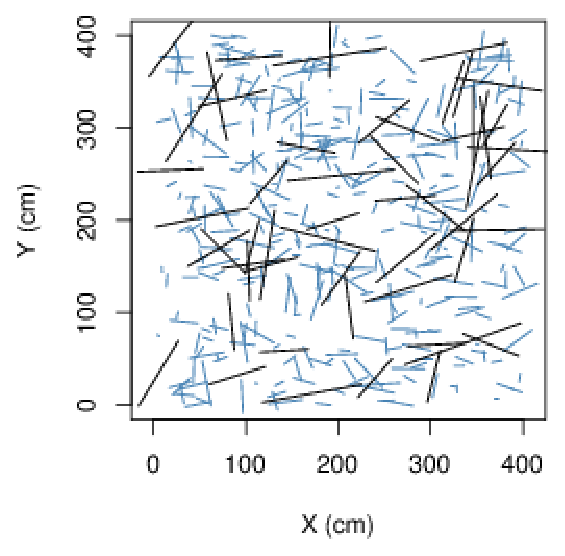
\includegraphics{fig11}
	\caption{DFN de una simulaci\'on de los datos. Comp\'arese con \autoref{f:dfn}.}
	\label{f:DFN_simInd}
\end{figure}

\subsection{El enfoque con la c\'opula de Bernstein}

La metodolog\'ia en esta secci\'on s\'i incluye la estructura de dependencia a trav\'es de la c\'opula de Bernstein de las pseudo-observaciones en la \autoref{f:scatterplot}. Con este modelo de c\'opula, se simularon nuevas pseudo-observaciones (izquierda de  la \autoref{f:alSim}) utilizando los pasos 1 y 2 del algoritmo de simulaci\'on bivariado. Despu\'es, utilizando el paso 3, se obtuvieron los valores simulados de orientaci\'on y longitud (derecha de la \autoref{f:alSim}) mediante las funciones cuantiles mostradas en la \autoref{f:cdfDL}.

La teor\'ia de c\'opulas permiti\'o tener las mismas marginales que en el caso independiente, es decir, la roseta de direcciones, el histograma de longitudes y los estad\'igrafos son exactamente los mismos que en el caso independiente. La diferencia radica en la estructura de dependencia. La \autoref{f:alSim} muestra los diagramas de dispersi\'on. N\'otese el contraste en aspecto visual de esta simulaci\'on comparada con los datos reales. Cuantitativamente, el coeficiente de correlaci\'on de rango ($\rho_M = 0.571$) tambi\'en es coherente con el de los datos.

\begin{figure}[H]
	\centering
	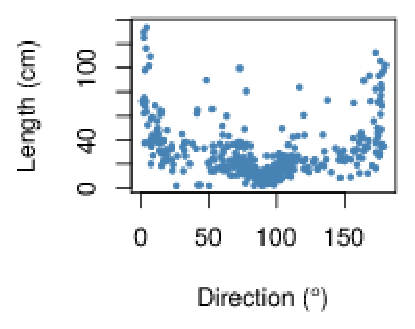
\includegraphics{fig12left}
	\qquad
	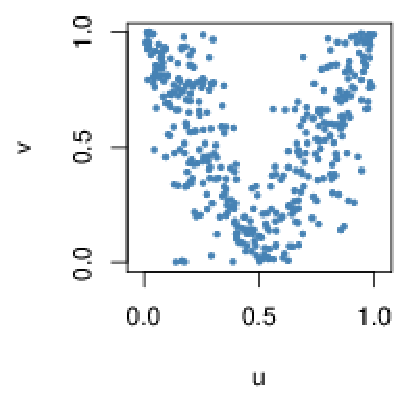
\includegraphics{fig12right}
	\caption{Diagrama de dispersi\'on y gr\'afico de pseudo-observaciones de la simulaci\'on que toma en cuenta la modelaci\'on de la estructura de dependencia. Comp\'arese con la \autoref{f:scatterplot} y con la \autoref{f:alSimInd}.}
	\label{f:alSim}
\end{figure}

La red de fracturas discretas correspondiente, al igual que en los datos sint\'eticos, muestra la preferencia de las fracturas m\'as largas por la direcci\'on N-S. Sin embargo, sin faltar a la realidad, todav\'ia existe la posibilidad de obtener fracturas en otras direcciones.

\begin{figure}[H]
	\centering
	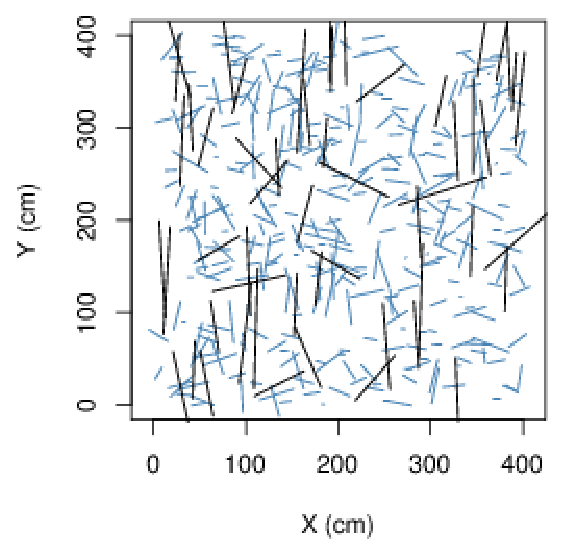
\includegraphics{fig13}
	\caption{DFN de la simulaci\'on basada en las c\'opulas de Bernstein. Comp\'arese con \autoref{f:dfn} y con \autoref{f:dfnSim}.}
	\label{f:dfnSim}
\end{figure}

